The primary aim of this analysis is to independently measure the rate
at which the Higgs boson is produced by VBF. This is carried out at
different Higgs signal mass hypotheses ($m_H$), and the Higgs
predictions from MC simulation are varied depending on the assumed $m_H$. Because
VBF and $VH$ define signal, and ggF is considered a background, both
signal and background templates change in the likelihood function for
different $m_H$. The best-fit $m_H$, as measured in the \hzz and \hgg
channels, is $125.36 \gev$. Therefore, this mass point is used as
a reference point.  

\subsection{$m_H = 125.36 \gev$}

\begin{figure}[h]
\centering
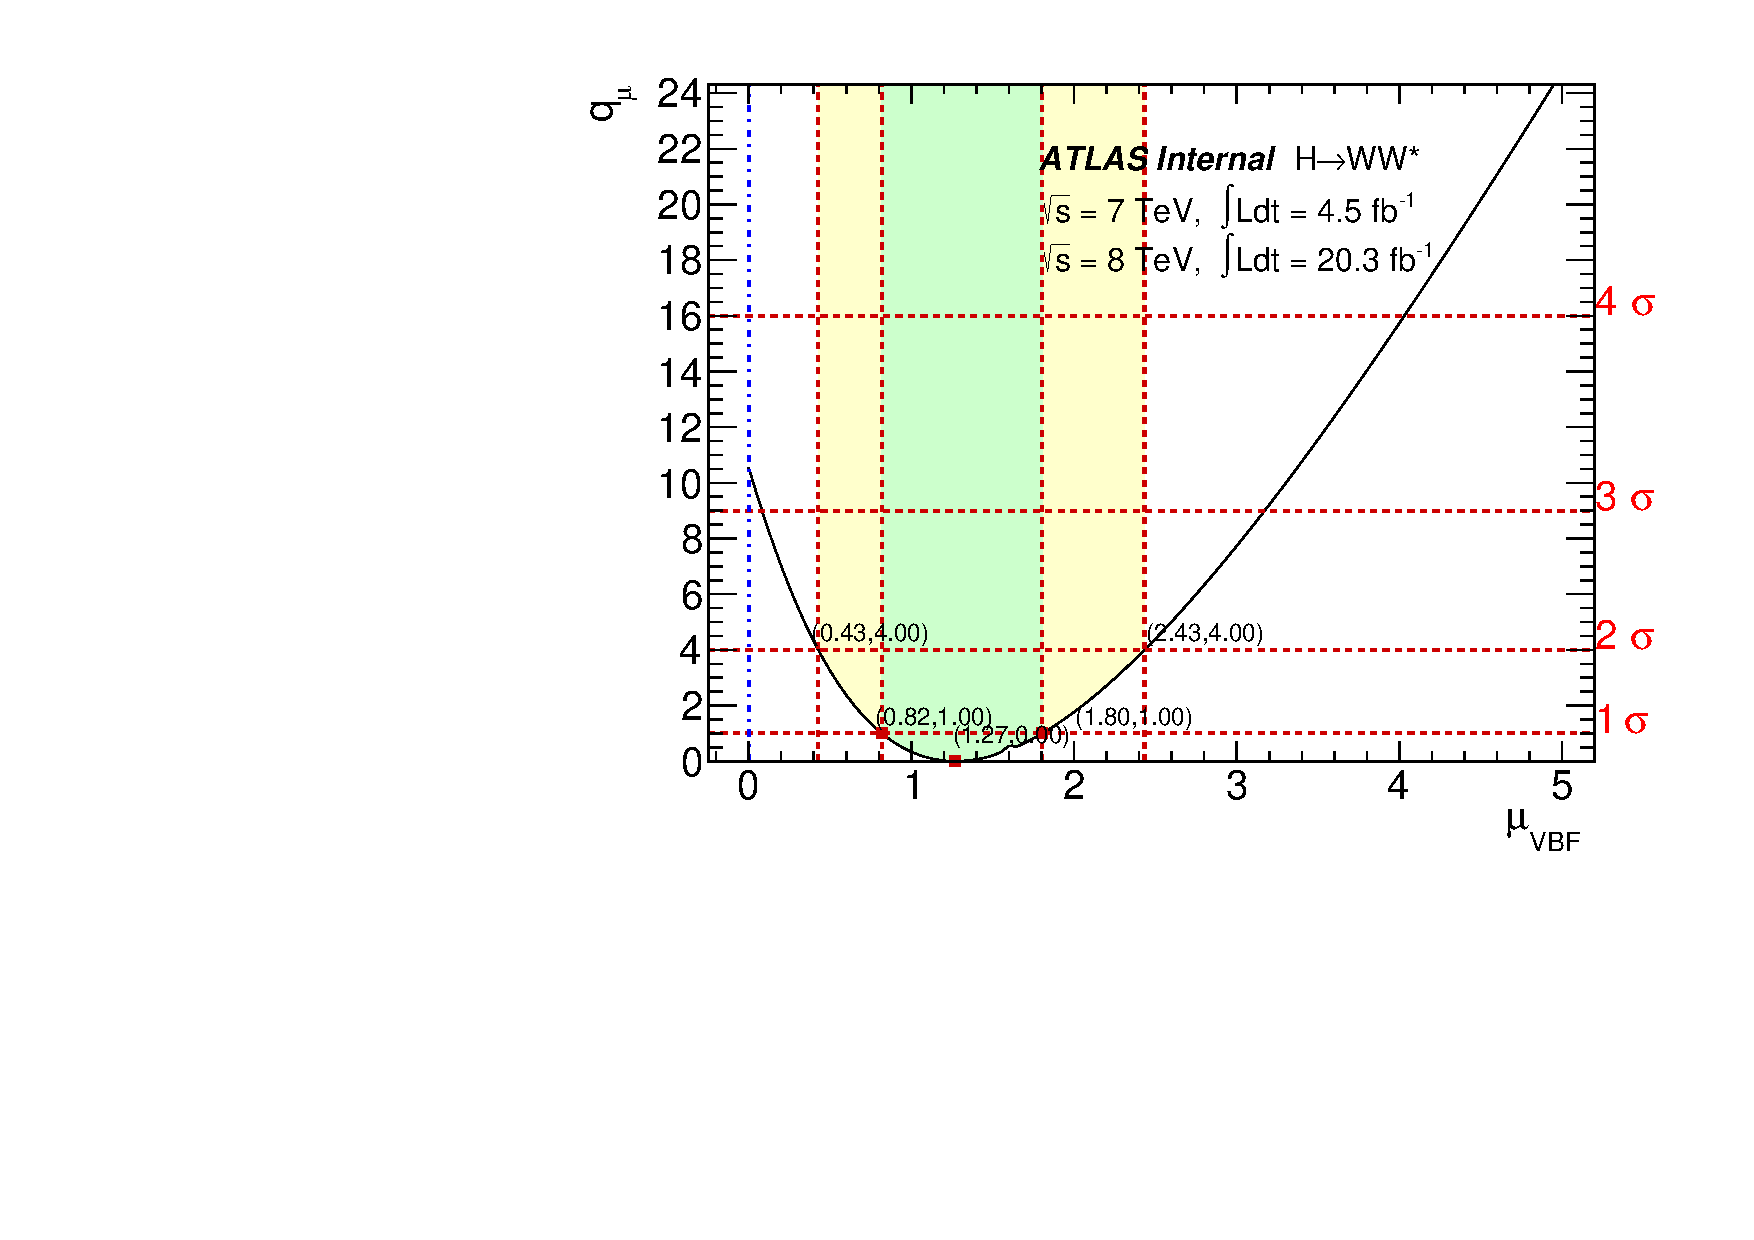
\includegraphics[width=0.6\textwidth]{fig/statistics/qmu_v_mu_combined.pdf}
\caption{Scan of the test statistic $q_{\mu}$ at different values of
$\mu$ at $m_H = 125.36 \gev$. The MLE of $\mu$ is obtained from the
minimum $q_{\mu}$, and the total error on $\hat{\mu}$ is obtained from
the $\mu$ points at which $q_{\mu} = 1$.}
\label{chap:analysis:fig:qmu_v_mu}
\end{figure}

The maximum likelihood estimate of $\mu_{\textrm{VBF}}$ is obtained by
maximizing $\mathscr{L}_{\textrm{full}}$, or equivalently, by
minimizing the
PLTS,
$q_{\mu}$~\ref{chapter:statistics:equation:test_statistic_runsig}. A
scan of $q_{\mu}$ as a function of $\mu$ is shown in
figure~\ref{chap:analysis:fig:qmu_v_mu} for $m_H = 125.36 \gev$. As
expected under the Wald approximation, the $q_{\mu}$ curve appears to be
parabolic. The
minimum is reached at $\hat{\mu} = 1.27$, a value which is larger than
the SM expectation due to the excess of observed events in the
$8 \tev$ SRs. The variance of $\mu$ is obtained from the
scan by interpolating the $\mu$ values at which $q_{\mu}=1$, resulting
in a $\sigma_+$ ($\sigma_-$) of 0.53 (0.45), or, splitting into
statistical and systematic uncertainty components:

\begin{equation}
\boxed{\hat{\mu}_{\textrm{VBF}} = 1.27^{+0.43}_{-0.39}\ (\textrm{stat})\
^{+0.30}_{-0.21}\ (\textrm{sys}) = 1.27^{+0.53}_{-0.45}\
(\textrm{total})}
\label{chapter:statistics:equation:observed_muhat_mH12536}
\end{equation}

\noindent
From the variance, it is evident that \muhat is consistent with the SM
expectation at $m_H = 125.36 \gev$. The best-fit value of the ggF
strength is exactly the SM expectation of 1.0, and the error is 20\%,
which, as shown in
table~\ref{chap:analysis:tab:sys_muhat_error_top15}, is one of the largest
contributions to the
total variance on $\mu_{\textrm{VBF}}$. 

In addition to to the variance,
the test statistic value $q_{0}^{\textrm{obs}}$ can be determined from
the scan. From
equation~\ref{chapter:statistics:equation:signif_discovery}, this
quantity is just the square of the observed
significance with which the null hypothesis is rejected, measured to be

\begin{equation}
\boxed{Z_0^{\textrm{obs}}\, (Z_0^{\textrm{exp}}) = 3.2\, (2.7)}
\label{chapter:statistics:equation:observed_signif_mH12536}
\end{equation}

\noindent
where the expected significance assuming $\muprime = 1$ is shown
parenthetically. This observed significance constitutes evidence of VBF Higgs boson
production at $m_H = 125.36 \gev$, as it is over the threshold of
$3\sigma$. Consistent with
$\hat{\mu}_{\textrm{VBF}}$, the observed $p_0$ falls within $1\sigma$
of the expected $p_0$ with $m_H = 125.36 \gev$. To quantify the
consistency with the SM, $Z_1^{\textrm{Obs.}}$ is computed, with the
result of $0.6\sigma$. In other words, assuming SM VBF production, an
experimental realization which is equally--- or less--- probable than
the one observed will be obtained in 28\% of identical
experiments. In contrast, the probability of the observation, assuming
that the data are distributed according to $\mu = 0$, is $7 \times
10^{-4}$. In
table~\ref{chap:statistics:tab:stats_muhat_signif}, $Z_0$ is split by
flavor channel and \sqrts. The excess over the $\mu = 1$
hypothesis is concentrated in the $8 \tev$ \eemm channel, where
$Z_0^{\textrm{obs}}$ ($Z_0^{\textrm{exp}}$) is 2.9 (1.3). This excess
is mitigated by the deficit in the $7 \tev$ analysis, in which 
$Z_0^{\textrm{obs}} = -1.0$ with $Z_0^{\textrm{exp}} = 0.9$.

\begin{table}
\begin{center}
\renewcommand{\arraystretch}{1.2}
\resizebox{0.5\textwidth}{!}{
\begin{tabular}{ l | c | c | c }
\hline
Channel & $\hat{\mu}$ & $Z_0^{obs}$ & $Z_0^{exp}$ \\
\hline
$7 \tev$ + $8 \tev$ & $1.3^{+0.7}_{-0.5}$ & 3.2 & 2.7 \\
\ \emme & $1.0^{+0.6}_{-0.5}$ & 2.4 & 2.3 \\
\ \eemm & $2.0^{+1.0}_{-0.8}$ & 2.7 & 1.3 \\
\hline
$8 \tev$ only & $1.5^{+0.6}_{-0.5}$ & 3.6 & 2.4 \\
\ \emme & $1.2^{+0.6}_{-0.5}$ & 2.7 & 2.2 \\
\ \eemm & $2.3^{+1.1}_{-0.9}$ & 2.9 & 1.3 \\
\hline
$7 \tev$ only & $-1.0^{+1.4}_{-1.1}$ & -1.0 & 0.9 \\
\hline
\end{tabular}
}
\caption[Statistical results at $m_H = 125.36 \gev$.]{The best-fit
signal strength and observed and expected significances with respect
to the null hypothesis at $m_H = 125.36 \gev$. Results are split by
flavor channel and \sqrts.}
\label{chap:statistics:tab:stats_muhat_signif}
\end{center}
\end{table}

\begin{table}[p!]
\begin{center}
%\renewcommand{\arraystretch}{1.2}
\resizebox{0.5\textwidth}{!}{
\begin{tabular}{l || c | c }
\hline
NP source & $\Delta \mu_{+\sigma}$ & $\Delta \mu_{+\sigma}$ \\
\hline
Statistical & +0.43 & -0.39 \\
$\textrm{JES}~\eta~\textrm{model}$ & +0.12 & -0.08 \\
Signal parton shower & +0.12 & -0.07 \\
$\mu_{\textrm{ggF}}$ & +0.09 & -0.08 \\
$\mathscr{B}_{\hww}$ & +0.09 & -0.05 \\
ABCD non-closure & +0.06 & -0.05 \\
Luminosity ($8 \tev$) & +0.06 & -0.04 \\
$WW$ QCD scale & +0.05 & -0.05 \\
Top $\alpha$ & +0.05 & -0.05 \\
Signal ME model & +0.07 & -0.04 \\
light tag SF & +0.06 & -0.04 \\
Signal PDF & +0.07 & -0.04 \\
ggF QCD scale & +0.04 & -0.04 \\
Top ME model (ggF) & +0.04 & -0.03 \\
ggF Higgs \pt~(0,1j) & +0.04 & -0.03 \\
\hline
Total Statistical & +0.43 & -0.39 \\
Total Systematic & +0.31 & -0.22 \\
Total & +0.53 & -0.45 \\
\hline
\end{tabular}
}
\caption[Top 15 NPs ranked by impact on $\hat{\mu}$ error and total
errors split into statistical and systematic components.]{The top 15
nuisance parameters ranked by impact on $\hat{\mu}$ error ($m_H = 125.36 \gev$), as well as
the total errors split into statistical and systematic components. Absolute
errors at $\pm 1\sigma$ are shown.}
\label{chap:analysis:tab:sys_muhat_error_top15}
\end{center}
\end{table}

In table~\ref{chap:analysis:tab:sys_muhat_error_top15}, the top 15 NPs
are ranked according
to their impact on $\hat{\mu}$. The impact of statistical
uncertainties is significantly larger than those associated with
systematic uncertainties. In fact, statistical uncertainties account
for 85\% of the total error on $\hat{\mu}$.

\subsection{Mass scan results}

Although $m_H$ has been measured in high resolution Higgs boson decay
channels, the rate of VBF Higgs production is independently measured
as a function of $m_H$ in the \wwlnln channel. In
table~\ref{chap:statistics:tab:mu_ggf_mu_vbf}, the best-fit VBF and
ggF signal strengths are shown for each test mass. At low $m_H$, both
$\hat{\mu}_{\textrm{VBF}}$ and
$\hat{\mu}_{\textrm{ggF}}$ are
significantly larger than the SM value, a consequence of the fact that
the $\mathscr{B}_{\hww}$ is an order of magnitude smaller than at the
reference
point. Without the ability to fully reconstruct the Higgs mass
from the decay products, the $m_H$ resolution suffers. Consequently,
any
excess over the null hypothesis at $m_H = 125.36 \gev$ leaks to
neighboring mass
points. This data excess, in concert with a smaller VBF and ggF
predictions at low $m_H$, pulls the best-fit strength parameters
up.

With $\mathscr{B}_{\hww}$ reaching a maximum at $m_H \sim 2 m_W$, the
errors on
$\mu_{\textrm{VBF}}$ and $\mu_{\textrm{ggF}}$ are minimized at $m_H$
points in this region. $\mu_{\textrm{ggF}}$ is measured to be
consistent with zero. $\mu_{\textrm{VBF}}$, on the other hand, is
consistently larger than 0, reaching a minimum at $m_H = 160 \gev$ of
$0.43 \pm 0.13$. This is an artifact of the especially poor mass
resolution in the VBF analysis. In the optimization of the BDT, mass
resolution has not been prioritized. Any mass resolution contribution
from the BDT input \mT is washed out by the other BDT inputs and the
coarse binning of the BDT response. Therefore, the signal template
does not vary
substantially with $m_H$, resulting in a large smearing
effect.

\begin{table}[h]
\begin{center}
%\renewcommand{\arraystretch}{1.2}
\resizebox{0.5\textwidth}{!}{
\begin{tabular}{l || c c}
\hline
$m_H$ (\gev) & $\hat{\mu}_{\textrm{VBF}}$ &
$\hat{\mu}_{\textrm{ggF}}$ \\
\hline
100 & $28.5^{+11.5}_{-9.91}$ & $12.96 \pm 5.79$ \\
105 & $14.0^{+5.59}_{-4.75}$ & $6.35 \pm 1.88$ \\
110 & $6.66^{+2.68}_{-2.26}$ & $3.68 \pm 0.79$ \\
115 & $3.45^{+1.42}_{-1.21}$ & $2.33 \pm 0.44$ \\
120 & $1.94^{+0.83}_{-0.7}$ & $1.52 \pm 0.29$ \\
125 & $1.31^{+0.54}_{-0.47}$ & $1.03 \pm 0.19$ \\
125.36 & $1.27^{+0.53}_{-0.45}$ & $1.0 \pm 0.19$ \\
130 & $0.92^{+0.38}_{-0.33}$ & $0.78 \pm 0.14$ \\
135 & $0.69^{+0.29}_{-0.25}$ & $0.57 \pm 0.12$ \\
140 & $0.59^{+0.24}_{-0.21}$ & $0.47 \pm 0.11$ \\
145 & $0.51^{+0.21}_{-0.18}$ & $0.4 \pm 0.09$ \\
150 & $0.46^{+0.18}_{-0.16}$ & $0.29 \pm 0.09$ \\
155 & $0.48^{+0.18}_{-0.15}$ & $0.13 \pm 0.06$ \\
160 & $0.43^{+0.15}_{-0.14}$ & $0.05 \pm 0.04$ \\
165 & $0.44^{+0.15}_{-0.13}$ & $0.03 \pm 0.03$ \\
170 & $0.48^{+0.17}_{-0.15}$ & $0.02 \pm 0.04$ \\
175 & $0.57^{+0.2}_{-0.17}$ & $0.01 \pm 0.04$ \\
180 & $0.68^{+0.23}_{-0.2}$ & $0.0 \pm 0.05$ \\
185 & $0.87^{+0.29}_{-0.26}$ & $0.0 \pm 0.06$ \\
190 & $0.98^{+0.34}_{-0.3}$ & $0.0 \pm 0.07$ \\
195 & $1.16^{+0.4}_{-0.35}$ & $0.0 \pm 0.09$ \\
200 & $1.28^{+0.44}_{-0.39}$ & $0.0 \pm 0.09$ \\
\hline
\end{tabular}
}
\caption[Best-fit $\mu_{\textrm{VBF}}$ and $\mu_{\textrm{ggF}}$ at
each $m_H$]{Best-fit $\mu_{\textrm{VBF}}$ and $\mu_{\textrm{ggF}}$ at
each $m_H$. Errors for the POI $\mu_{\textrm{VBF}}$ are computed with
the procedure described in
section~\ref{chap:statistics:sec:mu_hat_error}, while the error on
$\mu_{\textrm{ggF}}$ is derived from the Fisher information matrix. }
\label{chap:statistics:tab:mu_ggf_mu_vbf}
\end{center}
\end{table}

The observed $p_0$ is shown in
figure~\ref{chap:statistics:fig:signif_mH_injection_fullfit} as a
function of $m_H$. For comparison, the expected $p_0$ with the SM
signal expectation at $m_H = 125.36$ injected into the null hypothesis
is also shown. The observed
$p_0$ closely follows the expectation from an $m_H = 125.36 \gev$
signal--- though with an offset due to the excess--- over the entire
mass range. A maximum significance of $3.9\sigma$ is reached at $m_H =
190$. Again,
this is not surprising given the poor mass resolution and the fact
that a dominant background, ggF, is being scaled by its best-fit
value of $5 \times 10^{-5}$, the lowest measured
$\hat{\mu}_{\textrm{ggF}}$ value across the mass range. Similarly, at
$m_H > 160 \gev$, the expected significance for the injected signal is
greater than the expectation at the reference mass. 

\begin{figure}
\centering
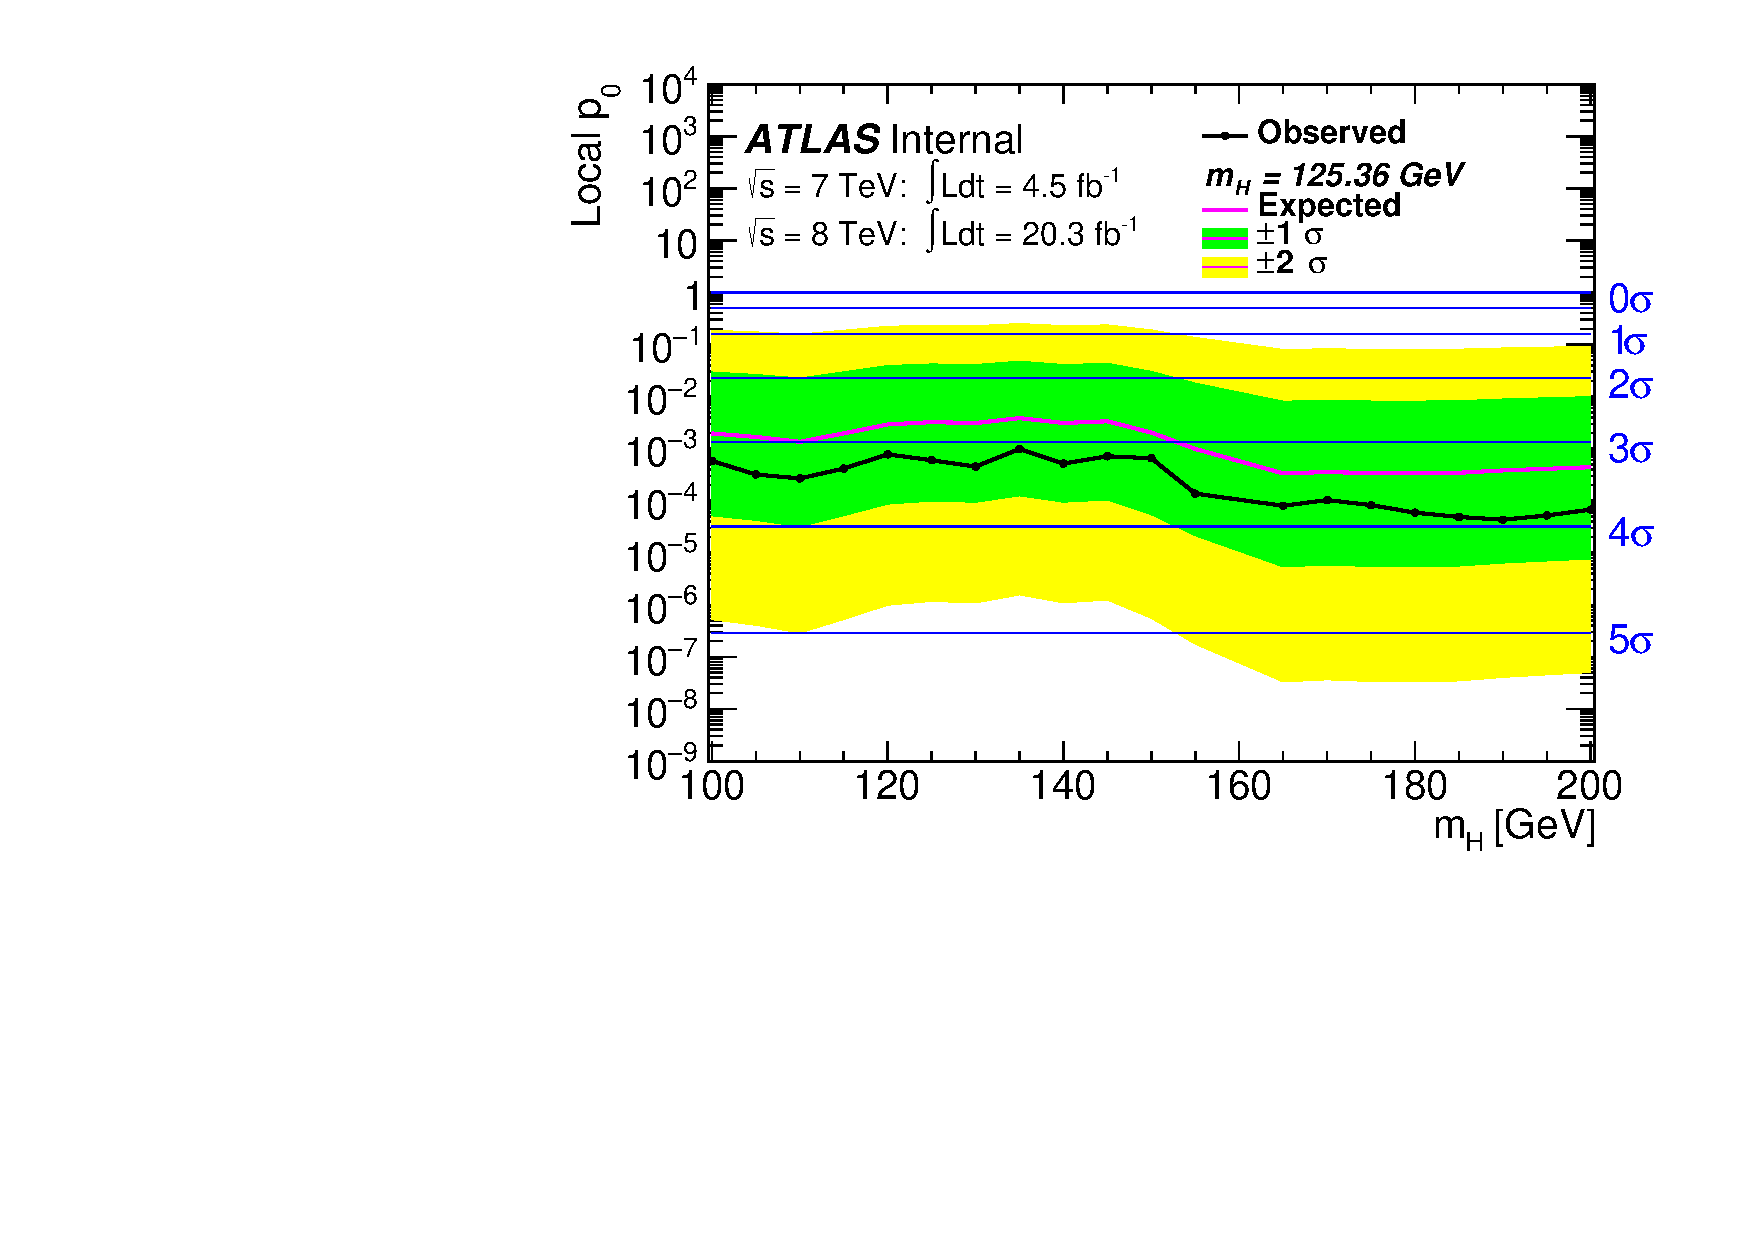
\includegraphics[width=0.6\textwidth]{fig/statistics/signif_plot/significance_mH_injection_ggF_profiled.pdf}
\caption{Significance plotted as a function of the Higgs mass
hypothesis. The observed p-value ($p_0^{\textrm{obs}}$) is shown in
black, and $p_0^{\textrm{exp}}$ with signal injected at $m_H =
125.36 \gev$ is shown in magenta. The $1\sigma$ ($2\sigma$) bands for
the $p_0^{\textrm{exp}}$ are shown in green (yellow). The associated
Z-score is shown in blue on the right vertical axis.}
\label{chap:statistics:fig:signif_mH_injection_fullfit}
\end{figure}
